%\section{Werkzeuge und Technologien}
%\label{sec:werkzeuge-und-technologien}

%\textit{Basierend auf dem Grundwissen über die Methoden und Praktiken, soll nun der Stand der Technik erörtert werden. Hierbei sollen Werkzeuge und Technologien und ihre Ansätze hervorgehoben werden und mit Hilfe welcher Methoden sie welches Ziel erreichen.}
%
%\textit{Wie in der Zielsetzung definiert sollen hier zwei bis drei Technologien näher vorgestellt werden.}
%
%\textit{Weiterhin könnte beleuchtet werden, wie ähnliche Herausforderungen bei anderen „Fat-Client“-Lösungen (also nicht SPAs) angegangen werden, und kann man hier vielleicht etwas lernen oder übertragen (und wenn nicht, warum nicht)?}

Um die gewünschte Lösung, den Proof-of-Concept, zu erstellen, muss zuvor der Stand der Technik erörtert werden. In diesem Abschnitt wird ein Überblick über aktuelle Technologien gegeben. Die vorgestellten Technologien werden kategorisiert und nach zuvor definierten Kriterien bewertet. Daraus ergibt sich eine Auswahl, der für den Proof-of-Concept in Frage kommenden Technologien.

\subsection{Recherche}

Um relevante und aktuelle Technologien zu ermitteln, wurde neben verfügbarer Literatur auch auf etablierte Plattformen bei der Gegenüberstellung von Technologien gesetzt. Dabei wurden Gartner\footnote{Gartner ist ein global agierendes Forschungs- und Beratungsunternehmen im Bereich der IT \cite{GartnerDefinition}} und StackShare\footnote{StackShare (\url{https://stackshare.io}) ist eine Vergleichsseite für Entwicklerwerkzeuge und Technologien, die auf Basis von Nutzereingaben Vergleiche erzeugt \cite{StackshareDefinition}} eingesetzt. Die identifizierten Technologien werden im nachfolgenden Abschnitt vorgestellt. 

Mithilfe von Gartners \enquote{Magic Quadrant for APM} \cite{GartnerMagicQuadrantForAPM} konnte festgestellt werden, dass folgende Werkzeuge zu den führenden Technologien in der Kategorie angehören: \textit{AppDynamics} \cite{AppDynamics}, \textit{Dynatrace} (ehemals ruxit) \cite{Dynatrace}, \textit{New Relic} \cite{NewRelic}, \textit{Broadcom DX APM} \cite{BroadcomDXAPM}, \textit{Splunk APM} \cite{SplunkAPM} sowie \textit{Datadog} \cite{Datadog}. Bestätigt werden einige dieser Technologien in der Bewertung bei StackShare \cite{StackShareAPM}. Hier sind insbesondere New Relic und Datadog zu erwähnen oft sowie  die Application Insights \cite{AzureApplicationInsights} des \textit{Azure Monitors} von Microsoft.

In der Literatur finden sich auch Vergleiche und Empfehlungen, so fanden z. B. Mart{\'i}nez \etal \cite{ComparisonOfE2ETestingToolsForMicroservices} in ihrer Evaluierung von Werkzeugen bei der Unterstützung von E2E-Tests, dass die beiden OpenSource-Technologien \textit{Jaeger} \cite{Jaeger} und \textit{Zipkin} \cite{Zipkin} aktiv dabei helfen können Fehlerszenarien in Microservice-Architekturen besser nachzuvollziehen. Weiterhin beschrieben Li \etal \cite{ServiceMeshChallengesStateOfTheArt}, wie mit \textit{Prometheus} \cite{Prometheus}, Jaeger, Zipkin und \textit{Fluentd} \cite{Fluentd} eine Datenanalyse von Microservices ermöglicht werden kann. Hinzukommend beschreiben Picoreti \etal \cite{MultilevelObservabilityInCloudOrchestration} eine Observability-Architektur, die auf Fluentd, Prometheus und \textit{Zipkin} basiert.

Bei StackShares Gegenüberstellung von Error-Monitoring-Produkten \cite{StackShareExceptionMonitoring} stechen drei Technologie heraus: \textit{Sentry} \cite{Sentry}, \textit{TrackJS} \cite{TrackJS} sowie \textit{Rollbar} \cite{Rollbar}. Die zwei erst genannten waren zudem auch bei der Gegenüberstellung der Monitoring-Lösungen \cite{StackShareMonitoring} gelistet.

StackShare bezeichnet Session-Replay als \enquote{User-Feedback-as-a-Service}. Hierbei \cite{StackShareUserFeedbackAsAService} lassen sich ebenfalls drei etablierte Produkte identifizieren: \textit{Inspectlet} \cite{Inspectlet}, \textit{FullStory} \cite{FullStory} und \textit{LogRocket} \cite{LogRocket}. Während Inspectlet und FullStory hauptsächlich auf die Nachvollziehbarkeit von User-Experience abzielen, konzentriert sich LogRocket auf technische Informationen, die für Entwickler von Bedeutung sind \cite{Webalyt}. Gartner bietet zudem eine Übersicht \cite{GartnerWebAndMobileAppAnalytics} über Produkte im \enquote{Web and Mobile App Analytics Market} an, in der sich \textit{Google Analytics} \cite{GoogleAnalytics}, \textit{Adobe Analytics} \cite{AdobeAnalytics} sowie LogRocket auf den obersten Positionen befinden.

\subsection{Übersicht}

In der \autoref{tab:technologie-uebersicht} werden nachfolgend die gefundenen Technologien näher veranschaulicht. Auf Basis der Produktbeschreibungen der Hersteller wird untersucht, welche Funktionalität die jew. Technologie vorweisen kann. Genauer werden folgende, zuvor identifizierte, Funktionalitäten unterschieden und den zugeordnet: IM, ASM, RUM, Error-Monitoring, Log-Management, (Distributed-)Tracing sowie Session-Replay. Um den Funktionsumfang zur jew. Funktionalität anzugeben, werden folgende 4 Schlüssel verwendet:

\begin{enumerate}
	\item \texttt{ja}: Die Funktionalität ist vorhanden und der Funktionsumfang entspricht der Definition.
	\item \texttt{ja(*)}: Die Funktionalität ist vorhanden, aber sie ist nicht so umfangreich wie bei anderen Technologien.
	\item \texttt{eingeschränkt}: Die Funktionalität ist nur unter bestimmten Voraussetzungen vorhanden oder ist nur teilweise implementiert.
	\item \textit{keine Angabe}: Die Funktionalität ist nicht vorhanden.
\end{enumerate}

\hvFloat[rotAngle=90,nonFloat=true,capWidth=w]%
{table}%
{
\begin{tabular}{|p{2.25cm}|p{1.5cm}|p{2.0cm}|p{3.0cm}|p{3.0cm}|p{1.5cm}|p{2.5cm}|}
\hline
Technologie & APM & RUM & Error-Mo\-ni\-tor\-ing & Log-Management & Tracing & Session-Replay \\
\hline
Adobe Analytics &  & gruppiert & teils &  &  &  \\
\hline
AppDynamics & ja & gruppiert & ja &  & ja &  \\
\hline
Broadcom DX APM & ja &  & teils & ja & ja &  \\
\hline
DataDog & ja & gruppiert & ja & ja & ja &  \\
\hline
Dynatrace & ja & gruppiert & ja & ja & ja &  \\
\hline
Elastic Stack & möglich & möglich & möglich & ja &  &  \\
\hline
Fluentd &  &  &  & ja &  &  \\
\hline
FullStory &  & ja & teils &  &  & ja \\
\hline
Google Analytics &  & gruppiert & teils &  &  &  \\
\hline
Graylog &  &  &  & ja &  &  \\
\hline
Inspectlet &  & ja & teils &  &  & ja \\
\hline
Jaeger &  &  &  &  & ja &  \\
\hline
LogRocket &  & ja & ja & teils &  & ja \\
\hline
New Relic & ja & gruppiert & ja & ja & ja &  \\
\hline
Papertrail &  &  &  & ja &  &  \\
\hline
\end{tabular}
}
{Übersicht der untersuchten Technologien, Teil 1}
{tab:technologie-uebersicht-teil1}

\hvFloat[rotAngle=90,nonFloat=true,capWidth=w]%
{table}%
{
\begin{tabular}{|p{2.25cm}|p{1.5cm}|p{2.0cm}|p{3.0cm}|p{3.0cm}|p{1.5cm}|p{2.5cm}|}
\hline
Technologie & APM & RUM & Error-Mo\-ni\-tor\-ing & Log-Management & Tracing & Session-Replay \\
\hline
Prometheus & ja &  &  &  &  &  \\
\hline
Rollbar &  & bei \mbox{Fehlern} & ja &  &  & teils \\
\hline
Sentry &  & bei \mbox{Fehlern} & ja &  &  &  \\
\hline
Splunk APM (SignalFX) & ja &  & ja &  & ja &  \\
\hline
Splunk \mbox{Enterprise} & möglich & möglich & möglich & ja &  &  \\
\hline
TrackJS &  & bei \mbox{Fehlern} & ja &  &  &  \\
\hline
Zipkin &  &  &  &  & ja &  \\
\hline
\end{tabular}
}
{Übersicht der untersuchten Technologien, Teil 2}
{tab:technologie-uebersicht-teil2}

\subsection{Kategorisierung}

Um die Veranschaulichung übersichtlicher zu gestalten, werden die Technologien auf Basis gemeinsamer Funktionalitäten kategorisiert. Auf Basis der evaluierten Funktionalitäten ergaben sich 6 Kategorien, in die die Technologien eingeordnet werden können. Diese Kategorien werden folgend erläutert:

\pagebreak

\begin{enumerate}
	\item APM-Plattformen
	\par Zu APM-Plattformen gehören allen voran Technologien, bei denen das Application-and-Service-Monitoring sowie das Infrastructure-Monitoring Kernfunktionalitäten darstellen. Bis auf ein Werkzeug begrenzen sich keine APM-Plattform nur auf diese beiden Aspekte, sondern können meist mehrere andere Funktionalitäten vorweisen. Am häufigsten sind Aspekte des Error-Monitorings, des Log-Managements sowie eines Distributed-Tracings vorzufinden. Neben technischen Aspekten bilden viele dieser Tools mithilfe von ASM und RUM auch Einsichten in die geschäftliche Leistung der Anwendung. Auf Basis von RUM wird teils Nutzerverhalten gruppiert visualisiert, um die Nutzerschaft besser verstehen zu können - eine Ansicht einer einzelnen Nutzersitzung wie beim Session-Replay ist jedoch nicht Teil dessen.
	
	\item Log-Plattformen
	\par Als Log-Plattformen werden alle Technologien bezeichnet, die eine Verarbeitung von Logdaten als ihre Kernfunktionalität verstehen. Nahezu alle hier angesiedelten Werkzeuge sind in der Lage Entwicklern und Betreibern eine detaillierte Analyse der Logdaten zu ermöglichen. Weiterhin steht oftmals die Funktionalität zur Verfügung diese Daten auch visuell Darstellungen zu können. Auf Basis der analytischen Funktionalitäten können zudem Aspekte von IM, ASM, RUM oder Error-Monitoring nachgestellt werden. Neben diesen Funktionalitäten steht aber auch ein effizientes Persistenzkonzept im Vordergrund, damit mit den enormen Datenmengen aus unterschiedlichen Systemen umgegangen werden kann \cite{TowardsAutomatedLogParsingForLargeScale}.
	
	\item Distributed-Tracing-Systeme
	\par Hiermit werden jene Technologien beschrieben, die ein Distributed-Tracing ermöglichen. Effiziente Architektur stehen oftmals im Vordergrund, welche explizit auf die enormen Datenmengen angepasst ist, die beim Distributed-Tracing anfallen können \cite{DapperInfrastructure}.
	
	\item Error-Tracking
	\par Die Kategorie Error-Tracking zeichnet sich dadurch aus, dass Technologien die Erhebung und Visualisierung von Fehlerdaten als ihre Kernfunktionalität verstehen. Weiterhin besitzen viele dieser Werkzeuge ein detailliertes Issue-Management, mit dem sich Teams organisieren können, um Fehler zu beheben und Arbeiten nachzuhalten.
	
	\item Session-Replay-Dienste
	\par Die Technologien der Kategorie Session-Replay zeichnen Nutzersitzungen auf und stellen diese Betreibern und Entwicklern in nachgestellter Videoform bereit. Hierbei lässt sich eine geschäftliche und eine technische Repräsentation unterscheiden. Bei ersterem werden Nutzersitzungen teils gruppiert und als Heatmaps dargestellt, bei letzterem werden detaillierte technische Informationen mitgeschnitten und dargestellt \cite{Webalyt}.
	
	\item Web-Analytics
	\par Die letzte Kategorie beschäftigt sich mit Web-Analytics-Technologien. Diese befassen sich mit der Evaluierung der Performance einer Webanwendung, sei es im geschäftlichen oder auch im technischen Sinne \cite{APracticalEvaluationOfWebAnalytics} \cite{WebAnalyticsAnHourADay}. Allgemeiner lässt sich anhand der Charakteristika sagen, dass Web-Analytics eine sehr spezifische Untermenge von APM-Plattformen darstellt.
	
\end{enumerate}

In der \autoref{tab:technologie-kategorisierung} werden die Technologien gruppiert nach ihrer Kategorie dargestellt. Da nicht alle Kategorien gleich hilfreich für die hier angestrebte Lösung sind, findet im \autoref{subsec:technologie-vorauswahl} eine Vorauswahl statt, welche Funktionskategorien näher betrachtet werden sollen.

\begingroup
\centering
\setlength{\LTleft}{-20cm plus -1fill}
\setlength{\LTright}{\LTleft}
\begin{longtable}{|p{4.10cm}|p{0.90cm}|p{0.90cm}|p{1.9cm}|p{1.75cm}|p{1.5cm}|p{1.4cm}|p{1.3cm}|}
\hline
Technologie & IM & ASM & RUM & Error-Montoring & Log-Mgmt. & Tracing & Session-Replay \\
\endhead
\hline
\hline
\multicolumn{8}{|l|}{APM-Plattformen} \\
\hline
AppDynamics & ja & ja & ja(*) & ja & eingeschr. & ja &  \\
\hline
Dynatrace & ja & ja & ja(*) & ja & ja & ja &  \\
\hline
New Relic & ja & ja & ja(*) & ja & ja & ja &  \\
\hline
Broadcom DX APM & ja & ja &  & teils & ja & ja &  \\
\hline
Splunk APM (SignalFX) & ja & ja &  & ja &  & ja &  \\
\hline
DataDog & ja & ja & ja(*) & ja & ja & ja &  \\
\hline
Azure Monitor & ja & ja &  & ja & ja & ja &  \\
\hline
Prometheus & ja & ja &  &  &  &  &  \\
\hline
\hline
\multicolumn{8}{|l|}{Log-Plattformen} \\
\hline
Papertrail & ja(*) & ja(*) & ja(*) & ja(*) & ja &  &  \\
\hline
Elastic Stack & ja(*) & ja(*) & ja(*) & ja(*) & ja &  &  \\
\hline
Fluentd &  &  &  &  & eingeschr. &  &  \\
\hline
Splunk \mbox{Enterprise} & ja(*) & ja(*) & ja(*) & ja(*) & ja &  &  \\
\hline
Graylog & ja(*) & ja(*) & ja(*) & ja(*) & ja &  &  \\
\hline
\hline
\multicolumn{8}{|l|}{Distributed-Tracing-Systeme} \\
\hline
Jaeger &  &  &  &  &  & ja &  \\
\hline
Zipkin &  &  &  &  &  & ja &  \\
\hline
\hline
\multicolumn{8}{|l|}{Error-Tracking} \\
\hline
Sentry &  &  & ja(*) & ja &  &  &  \\
\hline
TrackJS &  &  & ja(*) & ja &  &  &  \\
\hline
Rollbar &  &  & ja(*) & ja &  &  &  \\
\hline
Airbrake & ja & ja &  & ja &  &  &  \\
\hline
Bugsnag &  &  &  & ja &  &  &  \\
\hline
Raygun & ja & ja & ja(*) & ja &  &  &  \\
\hline
\hline
\multicolumn{8}{|l|}{Session-Replay-Dienste} \\
\hline
Inspectlet &  &  & ja & teils &  &  & ja \\
\hline
FullStory &  &  & ja & teils &  &  & ja \\
\hline
LogRocket &  &  & ja & ja &  &  & ja \\
\hline
\hline
\multicolumn{8}{|l|}{Web-Analytics} \\
\hline
Google Analytics & eing. & eing. & ja(*) & eingeschr. &  &  &  \\
\hline
Adobe Analytics & eing. & eing. & ja(*) & eingeschr. &  &  &  \\
\hline
\caption{Kategorisierung der untersuchten Technologien}
\label{tab:technologie-kategorisierung}
\end{longtable}
\endgroup


\subsection{Vorauswahl}
\label{subsec:technologie-vorauswahl}

Wie zuvor beschrieben eignen sich nicht alle Funktionskategorien teils mehr teils weniger für die, in dieser Arbeit angestrebte Lösung: Ein Proof-of-Concept, welches die Nachvollziehbarkeit einer Webanwendung von Anwendungsverhalten und Nutzerinteraktionen für \textbf{Betreiber und Entwickler} verbessert.

APM-Plattformen bieten durch ihr IM und ASM aufschlussreiche Einsichten in die Leistung und Verfügbarkeit einer Anwendung, helfen aber nicht oder kaum bei der Aufdeckung von einzelnen Problemen. Sie bieten hilfreiche Informationen aus wirtschaftlicher und operativer Sicht, bieten aber technische Informationen. Ein weiterer Grund gegen die Nutzung von Werkzeugen des Application-Performance-Monitorings ist die hier existierende Marktmacht von proprietären Lösungen. Die proprietären Ansätze zeichnen sich durch vorgefertigte Lösungen aus, die aber unflexibel in den Anpassungsmöglichkeiten sind. Um diese Diskrepanz näher zu untersuchen wurden New Relic und Dynatrace evaluiert. Hierbei konnte festgestellt werden, dass die bereitgestellten Informationen, aus Sicht eines Entwicklern, nicht ausreichend Aufschluss boten. So fehlte einedetaillierte Einsicht in einzelne Fehlerszenarien oder auch Nutzersitzungen. Stattdessen wurden gruppierte Informationen bereitgestellt, die die grobe \enquote{Gesundheit} des Systems widerspiegeln. Aus diesen Gründen, gerade aufgrund der divergierenden Zielgruppen, werden APM-Plattformen nicht näher betrachtet.

Aus einem ähnlichen Grund, wird die Kategorie Web-Analytics ebenso nicht näher behandelt. Werkzeuge im Web-Analytics-Bereich legen den Fokus sehr stark auf Überprüfung von wirtschaftlichen und operativen Eigenschaften, nicht jedoch den in dieser Arbeit erwünschten Zielen. Die übrig gebliebenen Kategorien werden im nächsten Unterabschnitt näher betrachtet und kriteriengeleitet bewertet.

\subsection{Kriterien}

Um für den Proof-of-Concept passende Technologien zu identifizieren, werden diese auf Basis verschiedener Kriterien bewertet. Diese Bewertung stützt sich auf öffentlich verfügbare Informationen, die die Hersteller der jeweiligen Technologie selber veröffentlicht haben. Die Kriterien werden folgend näher beschrieben.

\begin{enumerate}
	\item Kostenfrei
	\par Mit dem Kriterium \enquote{Kostenfrei} soll bewertet werden, ob eine kostenfreie Variante dieser Technologie existiert. Existiert eine kostenfreie Variante, wird \texttt{ja} angegeben und ansonsten \texttt{nein}. Existiert jedoch eine kostenfreie Version, die entweder von den Funktionalitäten oder der zeitlichen Nutzung beschränkt ist, wird diese mit \texttt{f. beschränkt} bzw. \texttt{z. beschränkt} angegeben.

	\item Support für Webanwendungen
	\par Bewertet, ob eine Unterstützung für das Senden von Daten von Webanwendungen existiert. Dies kann in der Form einer Anbindung (bsw. ein Agent\footnotemark{}) oder einer Schnittstelle sein. Ist eine Schnittstelle vorhanden, die aber nicht direkt aus einem Browserkontext ansprechbar ist, so ist diese Technologie mit \texttt{möglich} zu bewerten. Ist jedoch keine Schnittstelle vorhanden, die das Senden von eigenen Daten ermöglicht, so ist die Technologie mit \texttt{nein} zu bewerten.
		\footnotetext{Ein Agent ist eine Bibliothek, die die jeweiligen Daten (wie Klicks, Ladezeiten für Ressourcen und DOM-Events, usw.), eigenständig sammelt und an ein Partnersystem übertragt \cite{SolvingBigDataChallengesForAPM}}

	\item OnPremise und SaaS
	\par Mit diesen zwei Kriterien soll bewertet werden, wie diese Technologie eingesetzt werden kann. Ist sie in einer eigenen Infrastruktur aufsetzbar, also \enquote{On-Premise}, oder existiert die Technologie als buchbarer Dienst z. B. in der Cloud, also als Software-as-a-Service (SaaS).

	\item Standardisierung
	\par Setzt die jeweilige Technologie auf etablierte Standards, wie OpenTracing bei Distributed-Tracing? Falls nicht, sind einzelne Komponenten (z. B. zur Instrumentalisierung) quelloffen oder öffentlich spezifiziert, sodass diese ausgetauscht oder angepasst werden können.

	\item Multifunktional
	\par Mit dem Kriterium \enquote{Multifunktional} wird bewertet, ob eine Technologie neben der Kernfunktionalität auch weitere Funktionalitäten aufweist. Eine Technologie ist multifunktional, wenn sie min. zwei nicht nah verwandte Funktionalitäten nahezu vollständig besitzt (\texttt{ja} oder \texttt{ja(*)}). Nah verwandt sind hierbei IM und ASM.

	\item Zielgruppe
	\par Es ist einzuordnen, für welche Zielgruppen die Technologien einen Mehrwert bietet. Es werden folgende Zielgruppen differenziert: \texttt{Projektmanager}, \texttt{Fachabteilung} und \texttt{Entwickler}.
	
\end{enumerate}

Auf Basis dieser Kriterien werden nachfolgend die Technologien bewertet. Anschließend erfolgt für jede Kategorie eine Auswahl.

\subsection{Bewertung und Auswahl}
\label{subsec:bewertung-und-auswahl}

In der Kategorie \enquote{Log-Plattformen} findet sich auf Basis der Bewertung wenig Varianz zwischen den Technologien (vgl. \autoref{tab:technologie-bewertung-log-plattformen}), lediglich Fluentd sticht hervor. Dies ist dadurch erklärbar, dass Fluentd kein vollständiges Log-Management darstellt, sondern es sich um einen Logaggregator handelt \cite{FluentdAggregator}. Somit ist Fluentd nur als verwandte Technologie anzusehen und fällt somit als Präferenz aus. Der Elastic-Stack eignet sich durch die hohe Flexiblität und der Komponente Logstash auch dazu, Log-Management mit ihr zu betreiben  \cite{ThreatIdentificationFromAccessLogsUsingElasticStack} \cite{DesignLogManagementSystem}. Papertrail, Splunk sowie Graylog lassen sich als klassiche Log-Management-Werkzeuge verstehen, da sie speziell auf diese Funktionskategorie angepasst sind. Graylog sowie der Elastic-Stack sind quelloffen, aber auch als SaaS verfügbar. Bei einem gewünschten OnPremise Einsatz kann lediglich nur Papertrail nicht eingesetzt werden, denn dies wird nicht unterstüzt. Letztendlich lässt sich sagen, dass keine dieser vier Technologien ausschließende Eigenschaften besitzt, sondern allesamt für die in dieser Arbeit angestrebte Lösung geeignet sind.

Letztendlich wurde sich für \textbf{Splunk} entschieden, u. A. weil es beim Kunden bereits im Einsatz ist. Wie aber zuvor erwähnt, eignen sich die anderen Technologien ähnlich gut und eine erneute Auswahl mit anderen situationsbedingten Kriterien könnte variieren.

\begin{table}[H]%
\centering
\addtolength{\leftskip}{-2cm}
\addtolength{\rightskip}{-2cm}
\begin{tabular}{|p{3.05cm}|p{1.8cm}|p{1.7cm}|p{1.2cm}|p{1.3cm}|p{1.7cm}|p{1.3cm}|p{2.6cm}|}
\hline
Technologie & Kostenfrei & Support f. Webanw. & On \mbox{Premise} & SaaS & Standard. & Multif. & Zielgruppe \\
\hline
Papertrail & f. begrenzt & eingeschr. & nein & ja & nein & ja & Fachabteilung, Entwickler \\
\hline
Elastic Stack & ja & eingeschr. & ja & ja & eingeschr. & ja & Fachabteilung, Entwickler \\
\hline
Fluentd & ja & eingeschr. & ja & ja & eingeschr. & nein & Entwickler \\
\hline
Splunk \mbox{Enterprise} & f. begrenzt & eingeschr. & ja & ja & nein & ja & Fachabteilung, Entwickler \\
\hline
Graylog & ja & eingeschr. & ja & ja & eingeschr. & ja & Entwickler \\
\hline
\end{tabular}
\caption{Bewertung der Technologien der Kategorie \enquote{Log-Plattformen}}
\label{tab:technologie-bewertung-log-plattformen}
\end{table}


Im Gebiet der Distributed-Tracing-Systeme gibt es auch nur wenige oberflächliche Unterschiede (vgl. \autoref{tab:technologie-bewertung-distributed-tracing-systeme}). Sowohl Jaeger als auch Zipkin sind quelloffen und werden weitflächig eingesetzt \cite{AnalysisOfDistributedTracingSystemsEffectOnPerformance}. Jaeger scheint für neue Projekten attraktiver zu sein und findet dort mehr Einsatz, wie in StackShares Gegenüberstellung zu sehen ist \cite{StackShareJaegerVsZipkin}. Teilweise ist dies erklärbar durch die Ergebnisse, die Mart{\'i}nez \etal \cite{ComparisonOfE2ETestingToolsForMicroservices} herausfanden: Jaeger zeigt mehr hilfreiche Informationen an und kann diese schneller bereitstellen als Zipkin. Zudem entwickelt Jaeger aktiv eine Unterstützung des neuen OpenTelemetry-Standards \cite{JaegerOpenTelemetry}, bei Zipkin findet sich keine vergleichbare Entwicklung. Aus diesen Gründen ist \textbf{Jaeger} hierbei das Werkzeug der Wahl.

\begin{table}[H]%
\centering
\addtolength{\leftskip}{-2cm}
\addtolength{\rightskip}{-2cm}
\begin{tabular}{|p{3.05cm}|p{1.8cm}|p{1.7cm}|p{1.2cm}|p{1.3cm}|p{1.7cm}|p{1.3cm}|p{2.6cm}|}
\hline
Technologie & Kostenfrei & Support f. Webanw. & On \mbox{Premise} & SaaS & Standard. & Multif. & Zielgruppe \\
\hline
Jaeger & ja & eingeschr. & ja & nein & ja & nein & Entwickler \\
\hline
Zipkin & ja & eingeschr. & ja & nein & eingeschr. & nein & Entwickler \\
\hline
\end{tabular}
\caption{Bewertung der Technologien der Kategorie \enquote{Distributed-Tracing-Systeme}}
\label{tab:technologie-bewertung-distributed-tracing-systeme}
\end{table}


Die Auswahl in der Kategorie \enquote{Error-Tracking} ist etwas diverser (vgl. \autoref{tab:technologie-bewertung-error-tracking}), denn hier weisen manche Technologien Funktionalitäten auf, die sonst in dem Gebiet fremd sind. Bespielweise bieten Airbrake und Raygun neben einem Error-Monitoring zudem Aspekte eines APM, sodass die Anwendung/das System auch im Normalbetrieb überprüft werden kann. Diese APM-Funktionalitäten sind jedoch nicht so ausgereift, wie bei spezialisierten APM-Lösungen. Airbrake und Raygun sind lediglich als SaaS-Produkte, währenddessen Sentry, Rollbar und Bugsnag auch als OnPremise-Lösung verfügbar sind. Sentry ist zudem quelloffen auf GitHub \cite{GitHub} veröffentlicht\footnote{Sentry GitHub Repo: \url{https://github.com/getsentry/sentry}} und entwickelt dort mit der Community an dem Produkt weiter. Weiterhin ist Sentry das einzige identifizierte Werkzeug, welches eine nicht zeitlich begrenzte Version der SaaS-Lösung zur Verfügung stellt. Eine aussagekräftige Entscheidung kann jedoch nicht getroffen werden, da alle Werkzeuge des Error-Monitoring die gewünschten Anforderungen ausreichend erfüllen. Dennoch wird sich an dieser Stelle für \textbf{Sentry} entschieden, auf Basis der zuvor nahe gelegten Gründe.

\begin{table}[H]%
\centering
\addtolength{\leftskip}{-2cm}
\addtolength{\rightskip}{-2cm}
\begin{tabular}{|p{3.05cm}|p{1.8cm}|p{1.7cm}|p{1.2cm}|p{1.3cm}|p{1.7cm}|p{1.3cm}|p{2.6cm}|}
\hline
Technologie & Kostenfrei & Support f. Webanw. & On \mbox{Premise} & SaaS & Standard. & Multif. & Zielgruppe \\
\hline
Sentry & f. begrenzt & ja & ja & ja & eingeschr. & nein & Fachabteilung, Entwickler \\
\hline
TrackJS & z. und f. begrenzt & ja & nein & ja & nein & nein & Fachabteilung, Entwickler \\
\hline
Rollbar & z. und f. begrenzt & ja & ja & ja & nein & nein & Fachabteilung, Entwickler \\
\hline
Airbrake & z. und f. begrenzt & ja & nein & ja & nein & ja & Fachabteilung, Entwickler \\
\hline
Bugsnag & z. und f. begrenzt & ja & ja & ja & eingeschr. & nein & Fachabteilung, Entwickler \\
\hline
Raygun & z. und f. begrenzt & ja & nein & ja & nein & ja & Fachabteilung, Entwickler \\
\hline
\end{tabular}
\caption{Bewertung der Technologien der Kategorie \enquote{Error-Tracking}}
\label{tab:technologie-bewertung-error-tracking}
\end{table}


In der Beschreibung zur Kategorie \enquote{Session-Replay} wurde erwähnt, dass einige dieser Werkzeuge eine eher geschäfts- und andere eher eine entwicklerorientierte Session-Replay-Funktionalität vorweisen (vgl. \autoref{tab:technologie-bewertung-session-replay-dienste}). Genauer ist FullStory fast ausschließlich für das Nachvollziehen von User-Experience konzipiert, währenddessen LogRocket sehr detaillierte und sehr technische Informationen liefert \cite{Webalyt}. Inspectlet lässt sich als Mischung dieser beiden Sichten verstehen, bietet aber z. B. nicht alle Informationen an, die LogRocket darstellt  \cite{Webalyt}. Da die hier angestrebte Lösung auf Betreiber und insbesondere Entwickler abzielt, fiel die Wahl auf \textbf{LogRocket}.

\begin{table}[H]%
\centering
\addtolength{\leftskip}{-2cm}
\addtolength{\rightskip}{-2cm}
\begin{tabular}{|p{3.05cm}|p{1.8cm}|p{1.7cm}|p{1.2cm}|p{1.3cm}|p{1.7cm}|p{1.3cm}|p{2.6cm}|}
\hline
Technologie & Kostenfrei & Support f. Webanw. & On \mbox{Premise} & SaaS & Standard. & Multif. & Zielgruppe \\
\hline
Inspectlet & f. begrenzt & ja & nein & ja & nein & nein & Projektmanager, Fachabteilung, Entwickler \\
\hline
FullStory & f. begrenzt & ja & nein & ja & nein & nein & Projektmanager, Fachabteilung, Entwickler \\
\hline
LogRocket & f. begrenzt & ja & ja & ja & nein & nein & Fachabteilung, Entwickler \\
\hline
\end{tabular}
\caption{Bewertung der Technologien der Kategorie \enquote{Session-Replay-Dienste}}
\label{tab:technologie-bewertung-session-replay-dienste}
\end{table}


\subsection{Vorstellung der Technologien}

\subsubsection{Splunk}
\label{subsec:splunk}

Splunk bietet neben seiner akquirierten APM-Lösung (ehem. SignalFX) eine Log-Plattform an: Splunk Enterprise (nachfolgend einfach Splunk genannt). Dies stellt das Kernprodukt von Splunk dar und ist eine der führenden Plattformen auf dem Markt \cite{ThreatIdentificationFromAccessLogsUsingElasticStack}. Diese Lösung wird als OnPremise sowie auch als SaaS angeboten, was ein flexibles Deployment erlaubt.

Splunk bietet keine JavaScript-Bibliotheken, die das Senden von Daten an den Dienst vereinfachen - es steht jedoch mit dem HTTP Event Collector (HEC) \cite{SplunkHEC} eine Schnittstelle zur Verfügung, die eine Übermittlung von eigenen Logdaten ermöglicht. Der HEC ist standardmäßig nicht aus einem Browserkontext her verwendbar, da er mit ablehnenden CORS-Headern antwortet. Grund hierfür ist, dass der HEC nicht für dieses Szenario konzipiert wurde. Um dies zu umgehen, wurde ein Proxydienst eingerichtet, der die Daten des Frontends entgegennimmt, diese anreichert und dann an Splunk weiterleitet.

Auf Basis dieser Implementierung konnten alle Loginformationen eingesehen werden, sowie Fehlerdaten, welche zusätzlich an Splunk gemeldet wurden. Innerhalb von Splunk können mit der eigenen Search Processing Language (SPL) \cite{SplunkSPL} Abfragen durchgeführt werden (vgl. \autoref{fig:splunk_search-processing-language}). Mit dieser Sprache lassen sich, ähnlich wie bei SQL, einzelne Werte oder Listen abrufen aber auch neue komplexe Strukturen durch Unterabfragen generieren \cite{SplunkSQLtoSPL}.

\begin{figure}[H]
	\centering
	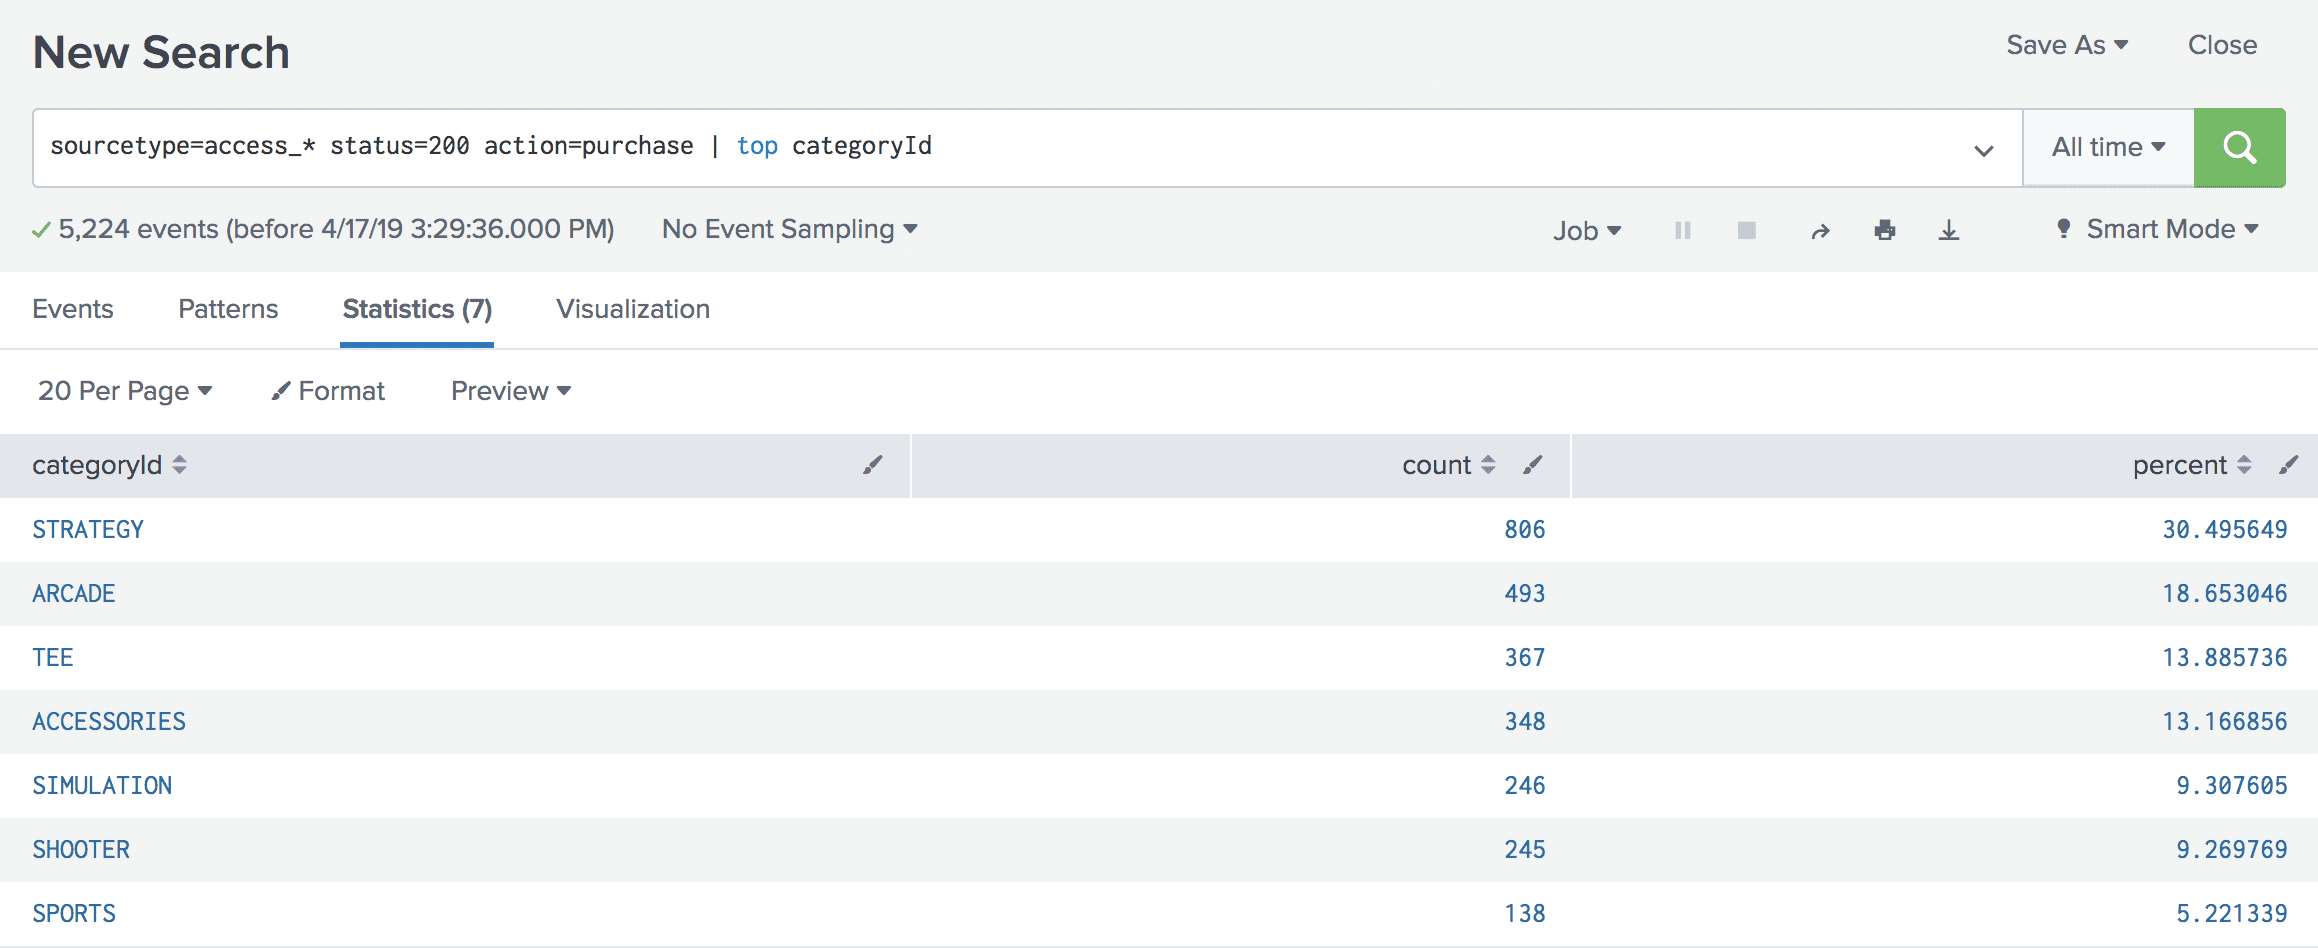
\includegraphics[width=\linewidth]{img/03_methoden/splunk_search-processing-language.png}
	\caption{Abfragebeispiel in Splunk aus \cite{SplunkSPL}}
	\label{fig:splunk_search-processing-language}
\end{figure}

\subsubsection{Jaeger}
\label{subsec:jaeger}

Jaeger wurde 2017 als ein OpenSource-Projekt der CNCF gestartet \cite{Jaeger}. Es ist ein System für verteiltes Tracing und bietet Funktionalitäten zur Datensammlung, --verarbeitung, und --speicherung bis hin zur Visualisierung. Jaeger unterstützt und implementiert den Standard OpenTracing, unterstützt aber auch Datenformate anderer Hersteller (wie z. B. Zipkin \cite{Zipkin}). Eine Unterstützung des OpenTelemetry-Standards ist derzeit in der Entwicklung. Darüber hinaus kann Jaeger genutzt werden, um Metriken nach Prometheus \cite{Prometheus} zu exportieren, einem weiteren CNCF-Projekt zur Speicherung und Visualisierung von Daten.

\begin{wrapfigure}[12]{r}{0.47\textwidth}
\centering
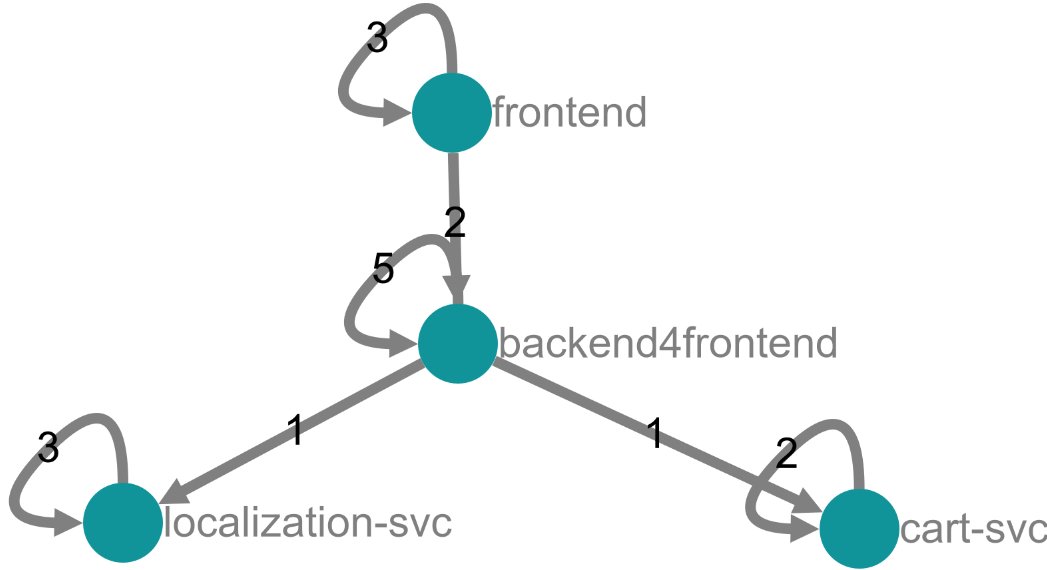
\includegraphics[width=\linewidth]{img/03_methoden/jaeger_dependency-graph.png}
\caption{Dienst-Abhängigkeits-Graph. Quelle: Eigene Darstellung}
\label{fig:jaeger-ui_dependency-graph}
\end{wrapfigure}

Jaeger spezialisiert sich auf Tracing und bietet hierfür eine skalierbare Infrastruktur zur Speicherung und Analyse der Daten. Die Traces werden als angereicherte Trace-Gantt-Diagramme dargestellt, wie in \autoref{fig:jaeger-ui_trace-detail-view} zu sehen ist. Hierbei werden sowohl hierarchische als auch zeitliche Beziehungen visualisiert. Wie bei OpenTracing und OpenTelemetry besteht ein Trace aus mehreren Spans, welche meist eine Methode umschließen. Zu den einzelnen Spans lassen sich weitere Informationen, wie bspw. Logmeldungen oder Kontextinformationen, anzeigen.

Anhand der Traces generiert Jaeger zudem automatisch eine Netzwerk-Topology, anhand der die Beziehungen zwischen Diensten nachvollzogen werden können (vgl. \autoref{fig:jaeger-ui_dependency-graph}).

\begin{figure}[H]
	\centering
	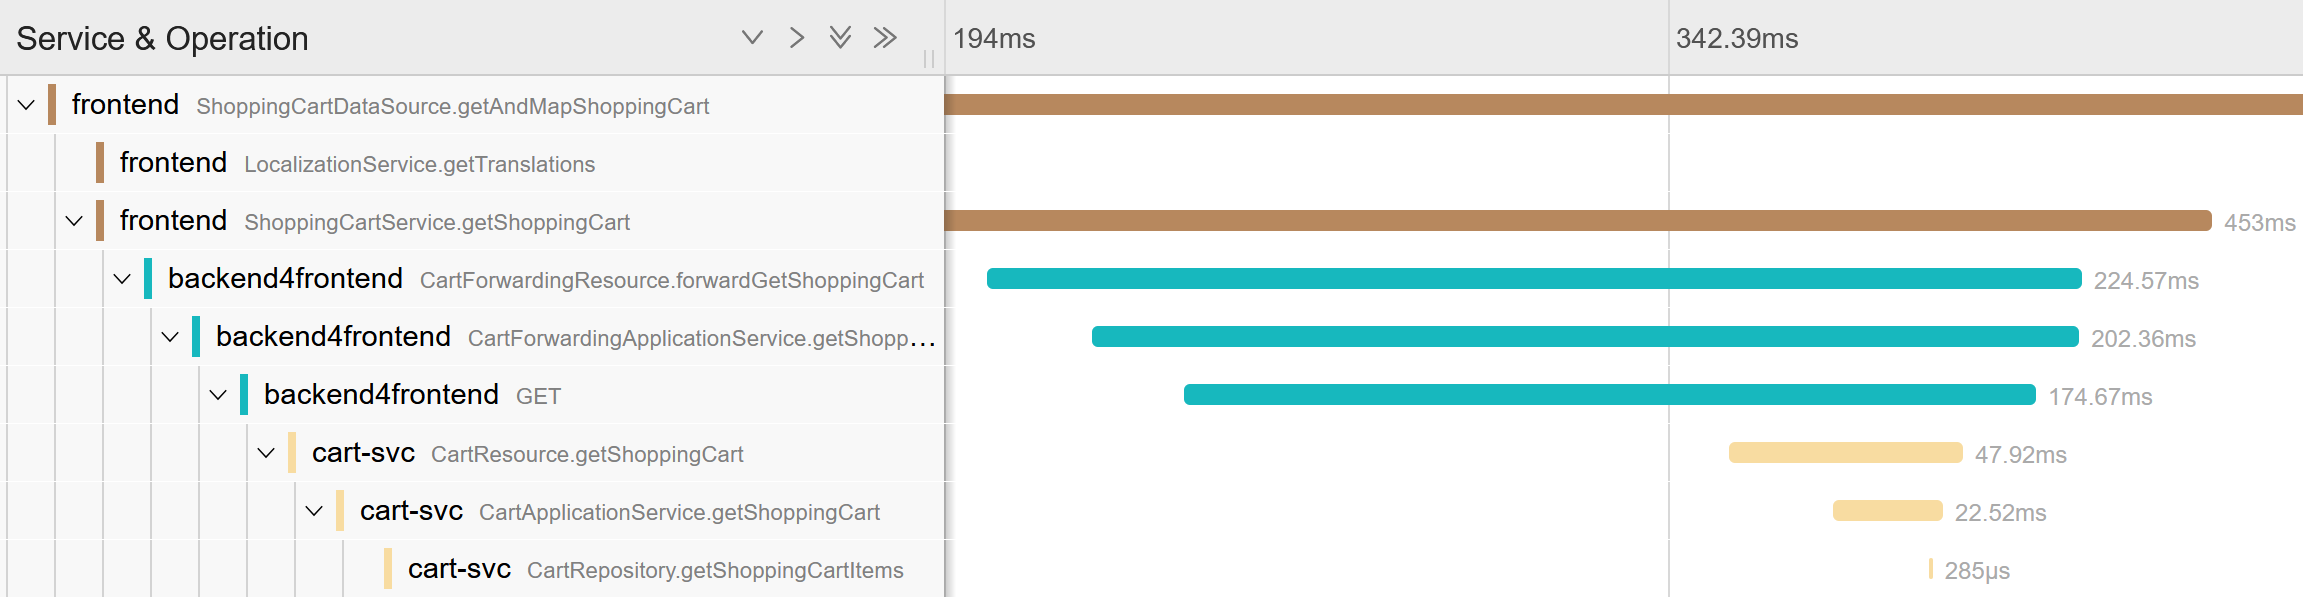
\includegraphics[width=\linewidth]{img/03_methoden/jaeger_trace-detail-view.png}
	\caption{Trace-Detailansicht. Eigener Screenshot aus Jaeger}
	\label{fig:jaeger-ui_trace-detail-view}
\end{figure}

\subsubsection{Sentry}
\label{subsec:sentry}

Sentry \cite{Sentry} ist ein SaaS-Produkt der Functional Software Inc., welches sich auf das Error-Monitoring spezialisiert. Die Kernfunktionalitäten beschränken sich auf das Error-Monitoring, auch wenn von anderen Praktiken einige Aspekte präsent sind, stellen diese keine eigens abgeschlossene Funktionalität dar.

Neben einer kommerziellen Version, stellt Sentry auch eine unbegrenzt kostenlos nutzbare Version bereit, welche im Rahmen dieser Arbeit evaluiert wurde. Der Quellcode für das Backend von Sentry ist, wie zuvor beschrieben, quelloffen verfügbar. Darüber hinaus wird zudem eine OnPremise-Lösung angeboten, die auf Docker basiert \cite{SentrySelfHosted}. Um von Webanwendungen Fehler zu erfassen und an Sentry zu melden, bietet Sentry bei NPM \cite{NPM} quelloffene Pakete an \cite{SentryJSGithub}. Dabei werden u. A. Anbindungen für folgende Technologien bzw. Frameworks bereitgestellt: JavaScript, Angular, React und Vue.js.

Wird ein Fehler gemeldet, erstellt Sentry hierzu ein \enquote{Issue}, also einen Problembericht. In einem Problembericht finden sich detaillierte Informationen zum Fehler, wie den Stacktrace, den Zeitstempel, die Nutzerumgebung (Browser, Version, etc.) sowie ein Ausschnitt der zuletzt aufgetretenen Logmeldungen in der Browserkonsole (vgl. \autoref{fig:sentry_issue-details}). Zudem schneidet Sentry jegliche Nutzerinteraktionen mit und stellt diese in dem Problembericht dar (vgl. \autoref{fig:sentry_issue-event-breadcrumbs}). Treten Fehler gleichen Ursprungs auf, fasst Sentry diese im selben Problembericht zusammen. Weiterhin kann jeder einzeln aufgetretener Fehler näher betrachtet werden.

Die angebotenen Fehlerinformationen von Sentry sind zahlreich und helfen beim Nachvollziehen besser als Logs und Traces allein. Eine ganzheitliche Nachvollziehbarkeit kann Sentry jedoch nicht anbieten, da die Informationen nur im Fehlerfall erhoben werden. Somit reicht Sentry nicht allein aus, um die in dieser Arbeit erwünschte Nachvollziehbarkeit zu erreichen.

\begin{figure}[H]
	\centering
	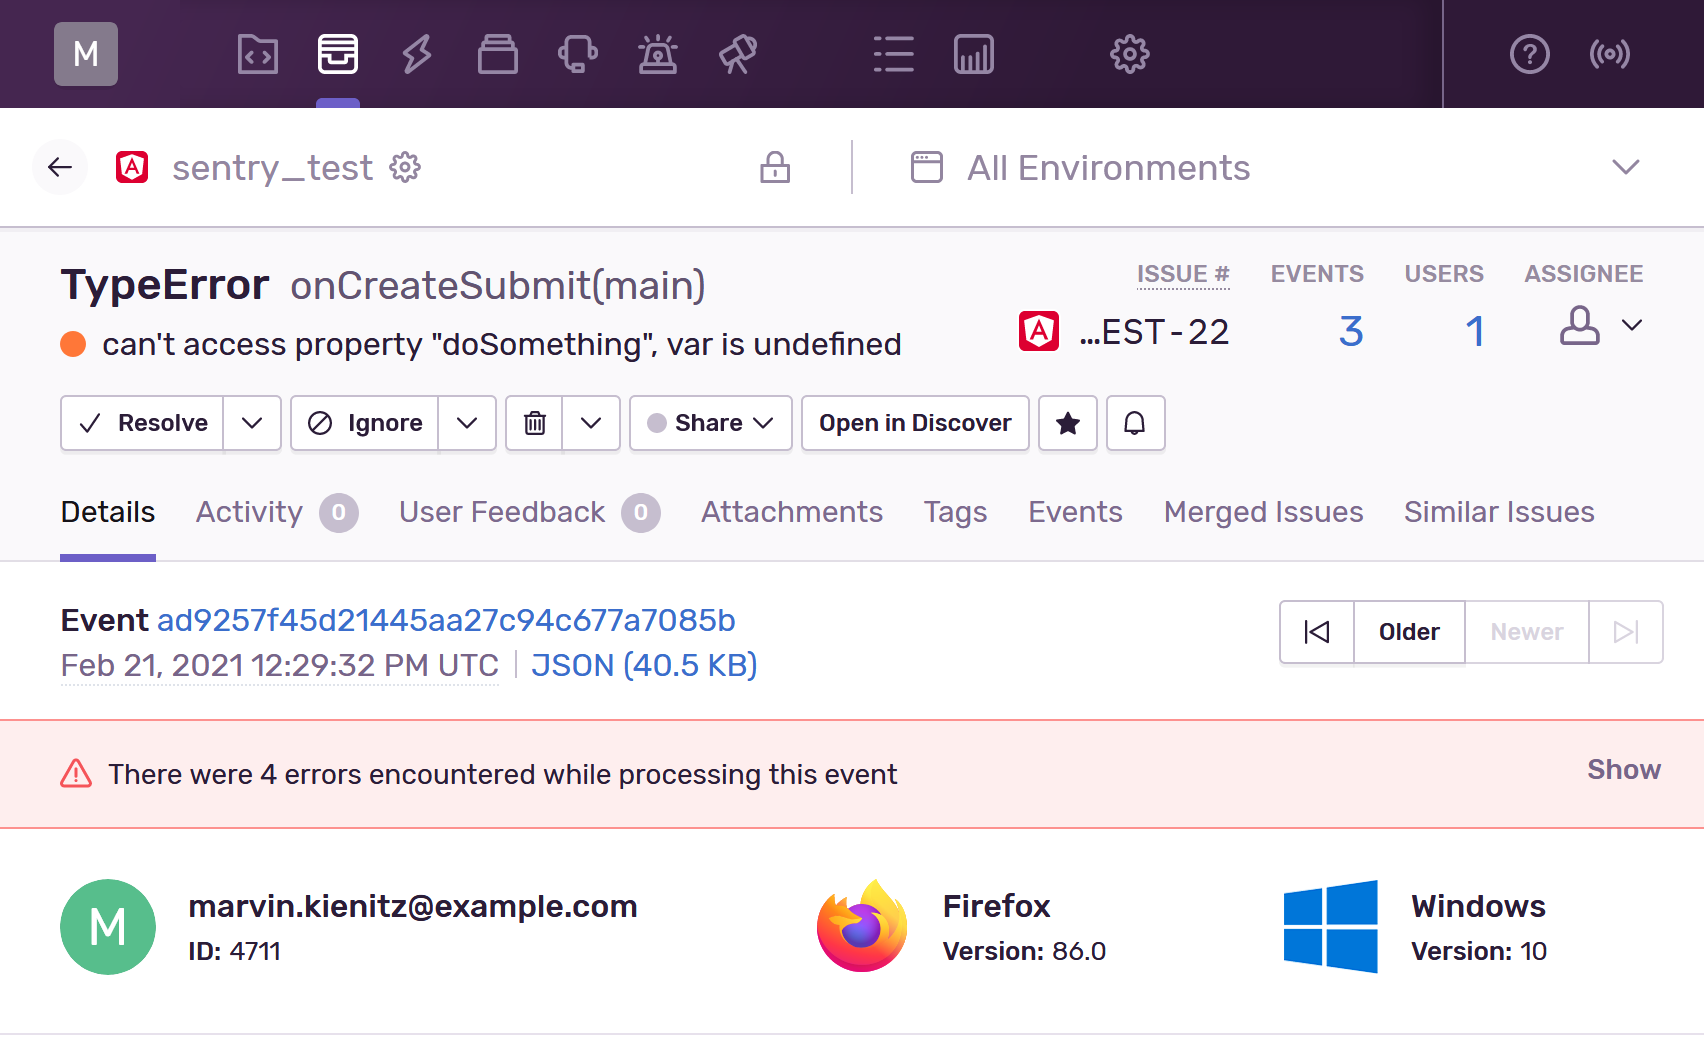
\includegraphics[width=1.00\linewidth]{img/03_methoden/sentry_issue-details.png}
	\caption{Kerninformation eines Issues. Eigener Screenshot aus Sentry}
	\label{fig:sentry_issue-details}
\end{figure}

\begin{figure}[H]
	\centering
	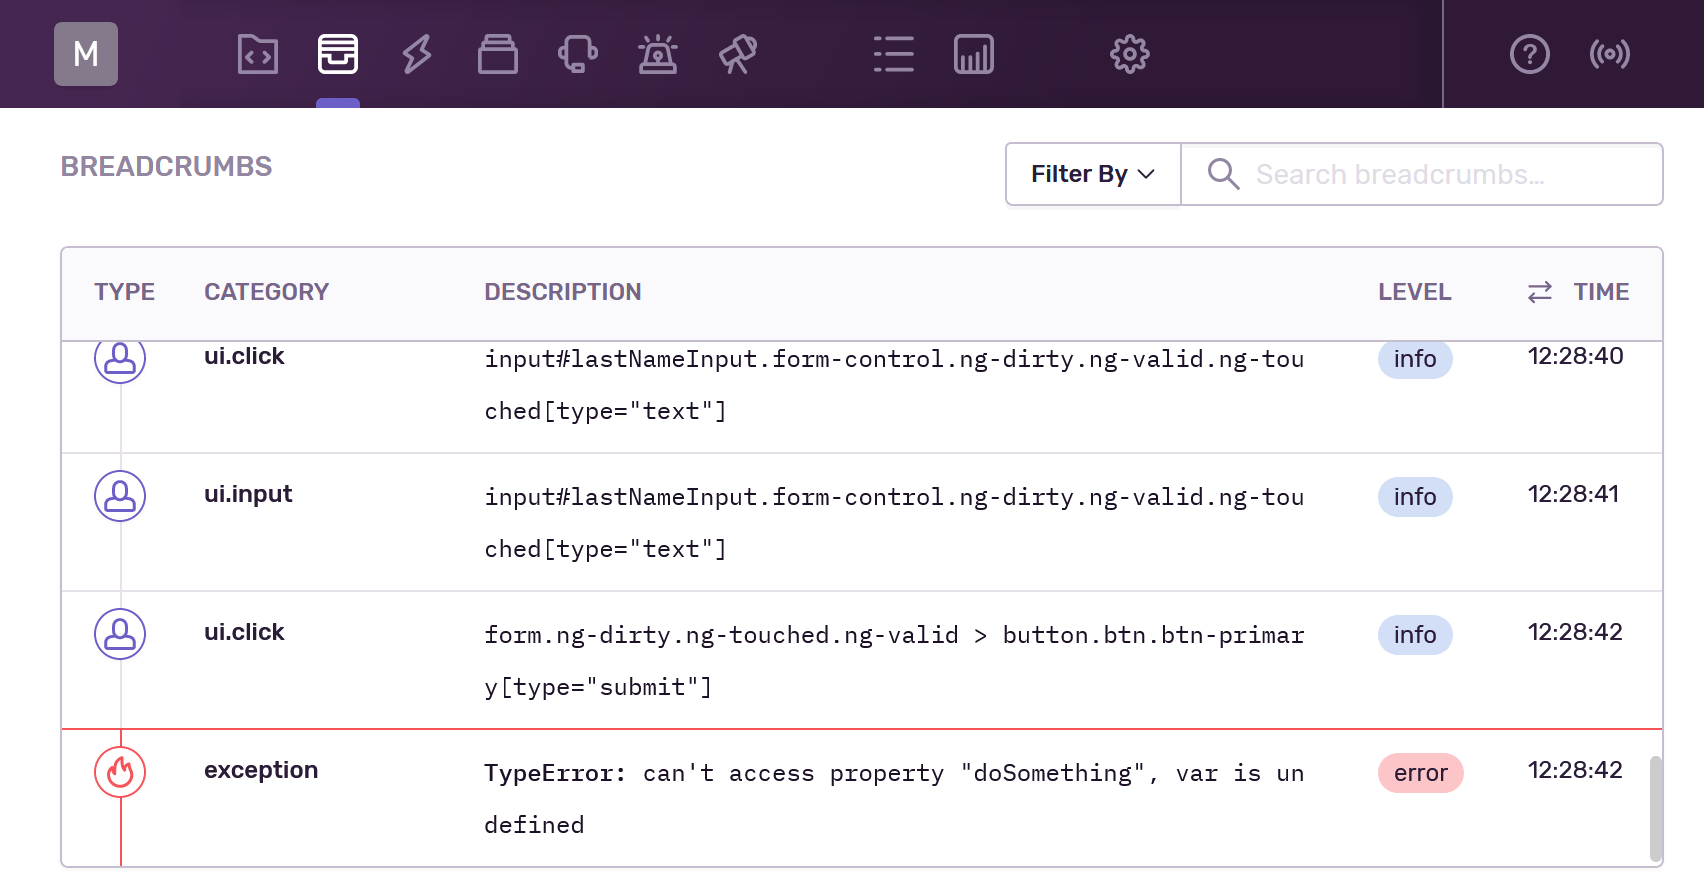
\includegraphics[width=1.00\linewidth]{img/03_methoden/sentry_issue-event-breadcrumbs.png}
	\caption{Verlauf der Userinteraktionen. Eigener Screenshot aus Sentry}
	\label{fig:sentry_issue-event-breadcrumbs}
\end{figure}

\subsubsection{LogRocket}
\label{subsec:logrocket}

LogRocket \cite{LogRocket} ist ein SaaS-Produkt des gleichnamigen Unternehmens und konzentriert sich auf detailliertes Session-Replay von JavaScript-basierten Clientanwendungen, um Probleme identifizieren, nachvollziehen und lösen zu können. Neben des SaaS-Produktes bietet LogRocket für Unternehmenskunden auch eine OnPremise-Lösung an. Anders als vergleichbare Session-Replay-Technologien nicht das Marketingteam o. Ä. \cite{Webalyt} die primäre Zielgruppe, sondern Entwickler.

LogRocket bietet eine kostenlose Testversion des SaaS-Produktes an, welche für die Evaluierung verwendet wurde. Zur Datenerhebung wird das Paket \texttt{logrocket} bei NPM \cite{NPM} angeboten, welches nach der Initialisierung eigenständig die notwendigen Daten sammelt. Mithilfe dieser Daten wird die gesamte Sitzung des Nutzers nachgestellt. Hierbei ist die Anwendung, die Nutzerinteraktionen, die Netzwerkaufrufe sowie das DOM zu sehen. Die Reproduktion wird videoähnlich aufbereitet und erlaubt ein präzises Nachvollziehen der zeitlichen Reihenfolge und Bedeutung (vgl. \autoref{fig:logrocket-session-replay-example}).

Neben dem JavaScript-SDK bietet LogRocket quelloffenene Plugins für folgende Bibliotheken: Redux, React, MobX, Vuex, ngrx, React Native. Zusätzlich bietet LogRocket auch eine Integration für andere Tools, wie z. B. Sentry. Bei der Integration für Sentry wird bei einem gemeldeten Fehler in Sentry direkt auf das \enquote{Video} in LogRocket verlinkt.

\begin{figure}[H]
	\centering
	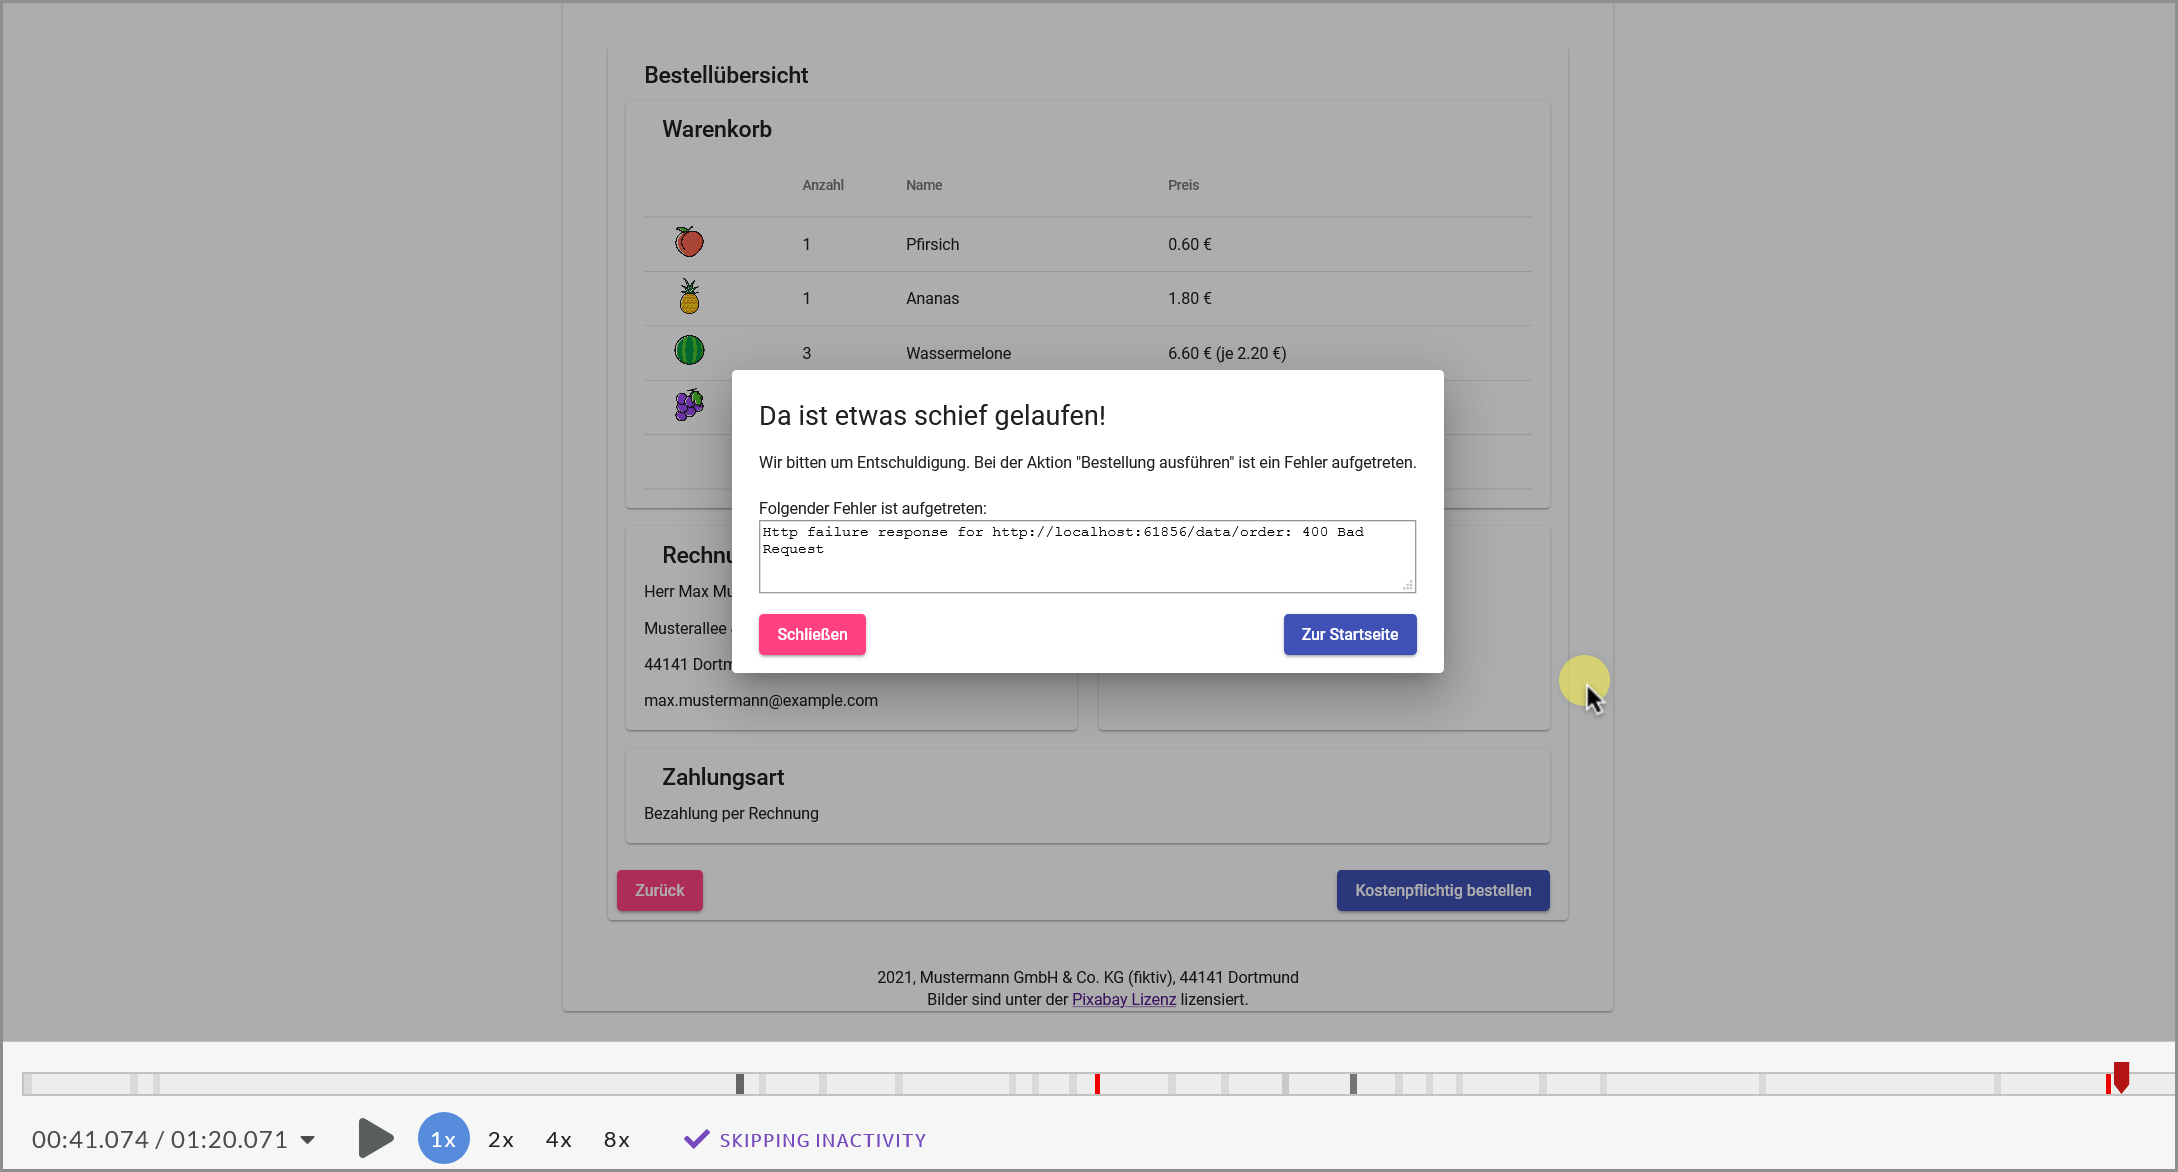
\includegraphics[width=\linewidth]{img/03_methoden/logrocket_session-replay-example-cropped.png}
	\caption{Ausschnitt eines Session-Replays. Eigener Screenshot aus LogRocket.}
	\label{fig:logrocket-session-replay-example}
\end{figure}